\chapter{Related Work}
\label{chap:related-work}

\section{Introduction}

This chapter surveys the literature in areas relevant to this thesis.
% TODO: First Section~\ref{sec:related-work-simplifying} provides a sample of non-machine learning-based approaches to lowering the cost of compiler construction. Subsequent sections provide a focused review of the specific topics of this thesis.
Section~\ref{sec:related-work-generation} reviews research in program generation, focusing first on generating benchmarks for performance characterisation, then compiler test case generation. Section~\ref{sec:related-work-optimisation} reviews the literature of empirical program optimisation, covering iterative compilation and machine learning. Section~\ref{sec:related-work-other} surveys the literature of related works in deep learning over programs. Finally Section~\ref{sec:related-work-summary} concludes.


% TODO:
%\section{\diff{Lowering the Cost of Compiler Construction}}
%\label{sec:related-work-simplifying}
%
%\diff{%
%Given the high cost of compiler construction (Table~\ref{tab:compiler-costs}), there has been much effort in reducing the complexity and engineering effort of constructing a compiler. One means for achieving this is through developing tooling for automatically generating compiler components from specifications. Popular examples include \emph{lex}~\cite{Lesk1975} for generating scanners, and \emph{yacc}~\cite{Johnson1975} for generating parsers. \citeauthor{Gray1992}~\cite{Gray1992} identify three chief limitations of this tooling approach: the steep curve for learning existing tools; tools which are developed independently and do not work smoothly together; and lower performance compared to hand-coded solutions to the same problems. They propose a system, \emph{Eli}, which decomposes the \emph{compilation problem} into discrete subproblems, provides reusable tools to solve each subproblem, and automatically combines the solutions into a working compiler. Compared to prior approaches, this system provides an end-to-end compiler generator from user-provided specifications. Delite~\cite{Sujeeth2014} and AnyDSL~\cite{Leißa2018} tackle the problem of lowering from high-level domain specific languages to performant low-level code such as CUDA, OpenCL, using .
%
%Does not address optimisation problems.
%
%The LLVM compilation framework~\cite{Lattner2004} takes a different approach. Rather than taking a user-specification and generating a compiler, it provides a common, low-level intermediate representation, an optimiser, and a set of re-usable components for lowering to machine code. LLVM has become one of the most widely used compilers in industry ,
%
%Frameworks such as these significantly reduce the engineering effort required to produce a compiler by simplifying the , however, they do not address the challenge of performance tuning.
%
%}


\section{Program Generation}
\label{sec:related-work-generation}

In this thesis, program generation is used as a mechanism to simplify the development of compiler heuristics and to validate the behaviour of compilers. The generation of artificial programs is a broad field with a wide range of applications; this section categorises the literature in the two areas that are relevant to this thesis: program generation for performance characterisation, and program generation for compiler validation.

\subsection{Benchmark Generation for Performance Characterisation}

Benchmark suites serve a wide variety of uses from compiler optimisations to hardware design. The challenge in creating a benchmark suite is to capture a diverse set of workloads that is both representative of real-world usage while providing adequate coverage of the program space. Achieving either of these two goals is a challenging task, and efforts towards one goal may hamper the other. As such, there is no ``one size fits all'' approach to assembling benchmark suites.

% Ryoo, J. H., Quirem, S. J., Lebeane, M., Panda, R., Song, S., & John, L. K. (2015). GPGPU Benchmark Suites: How Well Do They Sample the Performance Spectrum? ICPP.
Given its importance, benchmark suite characterisation has been the subject of much research. An evaluation of popular GPGPU benchmark suites~\cite{Ryoo2015} reveals there are important parts of the program space left untested.
% Xiong, W., Yu, Z., Bei, Z., Zhao, J., Zhang, F., Zou, Y., ... Xu, C. (2013). A Characterization of Big Data Benchmarks. In Big Data. IEEE. https://doi.org/10.1109/BigData.2013.6691707
\citeauthor{Xiong2013}~\cite{Xiong2013} demonstrate that workload behaviour is highly input dependent, and argue that benchmarks created for academic research cannot represent the cases of real-world applications.
% Ferdman, M., Adileh, A., Kocberber, O., Volos, S., Alisafaee, M., Jevdjic, D., ... Falsafi, B. (2012). Clearing the Clouds: A Study of Emerging Scale-out Workloads on Modern Hardware. In ASPLOS. ACM.
A review of big data benchmarks~\cite{Ferdman2012} found many to be unrepresentative, and that current hardware designs, while optimised for existing benchmark suites, are inefficient for true workloads.

% As well as covering the program space, benchmarks within suites should be diverse.
Benchmark suites should be \emph{diverse}, with each benchmark within a suite occupying a distinct point in the program space, else the benchmark may be redundant.
% Ould-Ahmed-Vall, E., Doshi, K. A., Yount, C., & Woodlee, J. (2008). Characterization of SPEC CPU2006 and SPEC OMP2001: Regression models and their transferability. In ISPASS. IEEE. https://doi.org/10.1109/ISPASS.2008.4510750
\citeauthor{Ould-Ahmed-Vall2008}~\cite{Ould-Ahmed-Vall2008} show that statistical models trained on 10\% of SPEC CPU 2006 data are transferable to the remaining data.
% Goswami, N., Shankar, R., Joshi, M., & Li, T. (2010). Exploring GPGPU workloads: Characterization methodology, analysis and microarchitecture evaluation implications. In IISWC. https://doi.org/10.1109/IISWC.2010.5649549
\citeauthor{Goswami2010}~\cite{Goswami2010} evaluate the diversity of 38 GPGPU benchmark workloads, finding that \emph{Similarity Score}, \emph{Scan of Large Arrays}, and \emph{Parallel Reduction} benchmarks show significantly different behaviour due to their large number of diverse kernels, but the remaining 35 benchmarks provide similar characteristics.
% Phansalkar, A., Joshi, A., & John, L. K. (2007). Analysis of redundancy and application balance in the SPEC CPU2006 benchmark suite. ACM SIGARCH Computer Architecture News, 35(2).
\citeauthor{Phansalkar2007}~\cite{Phansalkar2007} show that a subset of 14 SPEC CPU 2006 programs yields most of the information of the entire suite, and
% Panda, R., Song, S., Dean, J., & John, L. K. (2018). Wait of a Decade: Did SPEC CPU 2017 Broaden the Performance Horizon? In HPCA. IEEE.
\citeauthor{Draft2018}~\cite{Draft2018} find that SPEC CPU 2017 contains workloads that, when removed, do not degrade the suite's coverage of the program space.

Researchers have turned to \emph{synthetic} benchmarks to address the coverage and diversity challenges.
% Curnow, H. J., & Wichmann, B. A. (1976). A Syntetic Benchmark. Computer, 19(1).
The use of synthetic benchmarks is not new, with an early example from \citeyear{Curnow1976} using a synthetic benchmark to compare the computing power of processors for scientific workloads~\cite{Curnow1976}.
% Bell, R. H., & John, L. K. (2005). Improved automatic testcase synthesis for performance model validation. In SC. https://doi.org/10.1145/1088149.1088164
\citeauthor{Bell2005}~\cite{Bell2005} pose the \emph{synthesis} of synthetic benchmarks as a test case generation problem, using hardware counters to validate the similarity of synthesised benchmarks to a target workload.

% Joshi, A. M., Eeckhout, L., Johnz, L. K., & Isen, C. (2008). Automated microprocessor stressmark generation. In HPCA.
A popular use of synthetic benchmark generation techniques is to aid microprocessor design. \citeauthor{Joshi2008}~\cite{Joshi2008} use micro-architecture-independent characteristics such as basic block sizes and data footprint to summarise workloads. Their benchmark generator, \emph{BenchMaker}, then generates a linear sequence of basic blocks and randomly populates them with assembly instructions to match the desired workload characteristics.
% Bertran, R., Buyuktosunoglu, A., Gupta, M. S., Gonzalez, M., & Bose, P. (2012). Systematic Energy Characterization of CMP/SMT Processor Systems via Automated Micro-Benchmarks. In MICRO. IEEE.
\emph{MicroProbe}~\cite{Bertran2012} uses feedback-directed micro-benchmark generation to perform a systematic energy characterisation of a processor.

\emph{GENESIS}~\cite{Chiu2015} is a language for generating synthetic training programs. The essence of the approach is to construct a probabilistic grammar with embedded semantic actions that define a language of possible programs. New programs may be created by sampling the grammar and, through setting probabilities on the grammar productions, the sampling is biased towards producing programs from one part of the space or another. Theoretically, this technique is completely general since a grammar may be constructed to match any desired program domain. However, despite being theoretically possible, it is not easy in practice to construct grammars which are both suitably general and also produce programs that are in any way similar to what humans write. Such grammar-based benchmark generators have been shown to be successful only over a highly restricted space of stencil benchmarks with little control flow or program variability~\cite{Garvey2015b,Falch2015,Cummins2016a}. Restricting the domain of programs that can be generated limits the usefulness of this approach for many problems. It remains unclear how much effort it would take to define grammars capable of producing realistic programs in more complex domains.

Interesting recent developments in synthetic benchmark generation have combined elements from feedback-directed test case synthesis (reviewed in the next section) with synthetic benchmarking for the purpose of generating \emph{adversarial} benchmarks that expose performance issues in systems.

% Dhok, M., & Ramanathan, M. K. (2016). Directed Test Generation to Detect Loop Inefficiencies. In FSE. ACM.
\citeauthor{Dhok2016}~\cite{Dhok2016} apply mutation techniques to an initial set of coverage-driven inputs to expose inefficiencies in loops.
% Petsios, T., Zhao, J., Keromytis, A. D., & Jana, S. (2017). SlowFuzz: Automated Domain-Independent Detection of Algorithmic Complexity Vulnerabilities. In CCS. ACM.
\emph{SlowFuzz}~\cite{Petsios2017} uses resource-usage to guide evolutionary search over program inputs to expose performance bottlenecks that could be exploited by attackers to produce Denial-of-Service attacks. It considers the input to a program as a byte sequence and performs mutations to find the byte sequence within a fixed input size that maximises slowdown.
% Wei, J., Chen, J., Feng, Y., Ferles, K., & Dillig, I. (2018). Singularity: Pattern Fuzzing for Worst Case Complexity. In ESEC/FSE. ACM.
Similarly, \emph{Singularity}~\cite{Wei2018} uses an evolutionary search over the space of program inputs but using input \emph{patterns} to find the input with the worst case performance.

% Toffola, L. D., Pradel, M., & Gross, T. R. (2018). Synthesizing programs that expose performance bottlenecks. In CGO.
\emph{PerfSyn}~\cite{Toffola2018} tackles the related problem of exposing performance bottlenecks from API usage. For a method under test, it starts with a minimal example input and applies a sequence of mutations that modify the original code.
% Lemieux, C., Padhye, R., Sen, K., & Song, D. (2018). PerfFuzz: Automatically Generating Pathological inputs. In ISSTA. ACM. https://doi.org/10.1145/3213846.3213874
\emph{PerfFuzz}~\cite{Lemieux2018} uses feedback-directed program mutation to generate programs which maximise execution counts at program locations.
% Pedrosa, L., Iyer, R., Zaostrovnykh, A., Fietz, J., & Argyraki, K. (2018). Automated Synthesis of Adversarial Workloads for Network Functions. In SIGCOMM. ACM. https://doi.org/10.1145/3230543.3230573
\citeauthor{Pedrosa2018}~\cite{Pedrosa2018} applies the adversarial benchmark approach to network functions. Their tool, \emph{CASTAN}, takes as input the code for a network function and outputs packet sequences that trigger slow execution paths.

\citeauthor{Ding2019}~\cite{Ding2019} propose an alternate approach to addressing data scarcity in machine learning. Instead of generating benchmarks whose features must be evaluated and labelled to derive training data, they instead generate new feature values and labels based on the distributions in the training set. In contrast to the methods proposed in this work, their dataset generator --- based on a Gaussian Mixture Model --- is explicitly designed to amplify unusual behaviour within the training set. The generative model proposed in this work is intended to produce new data that is representative of the training set.

In contrast to prior works, the benchmark generation technique proposed in this thesis provides \emph{general-purpose} program generation over unknown domains, in which the statistical distribution of generated programs is automatically inferred from a corpus of real-world code. This allows \emph{representative} benchmarks to be generated automatically without expert guidance. To the best of my knowledge, no prior work has tackled the problem of undirected benchmark generation from example code.


\subsection{Test Case Generation for Compiler Validation}

Compilers are a fundamental trusted technology, and their correctness is critical. Errors in compilers introduce security vulnerabilities and catastrophic runtime failures. Therefore, ensuring that a compiler behaves as expected is of utmost importance.

Approaches to assure compiler behaviour are divided into \emph{verification} and \emph{validation}. The complexity of optimising compilers and the programming languages they compile renders formal verification of the entire compiler prohibitively expensive. Efforts have been made in this direction, for example, CompCert~\cite{Leroy2013}, a formally verified compiler for the C programming language, but this comes at the cost of supporting only a subset of the language features and with significantly lower performance compared to unverified compilers such as GCC~\cite{Daniel2017}. Still, even CompCert is not fully verified, and errors have been discovered in the unverified components~\cite{Yang2011}.

Because of the difficulties of \emph{verification}, compiler developers turn to \emph{validation}, in which the behaviour of a compiler is validated using a set of handcrafted input programs, or \emph{test cases}. For each test case, the expected outcome (determined by the specification of the compiler) is compared against the observed outcome to validate that the compiler conforms to the specification, for those inputs. However, the absence of errors during the validation process does not prove that the compiler is free from errors unless all possible inputs are tested exhaustively, and the input space for compilers is huge\footnote{In theory, the input space of a compiler is infinite. In practice, however, constraints such as maximum input file size bound the space, though to all intents and purposes an exhaustive validation of a compiler's input space is intractable.}. As such, hand-designed suites of test programs, while important, are inadequate for covering such a large space and will not touch all parts of the compiler.

The random generation of programs to test compilers is a well-established approach to the compiler validation problem. The main question of interest is in how to efficiently generate programs which expose bugs. There are two main approaches: \emph{program generation}, where inputs are synthesised from scratch; and \emph{program mutation}, where existing codes are modified so as to identify anomalous behaviour. These approaches are reviewed in turn.


\subsubsection{Program Generation for Compiler Testing}

The idea of generating programs to test compilers is well-established. The majority of test case generation approaches are based on a formal specification of the programming language syntax and grammar.
% Hanford, K. V. (1970). Automatic Generation of Test Cases. IBM Systems Journal, 9(4).
An early approach is presented by \citeauthor{Hanford1970a}~\cite{Hanford1970a}, which randomly enumerates programs described by a context-free grammar to produce an inexhaustible supply of new programs. While the generated programs are syntactically valid, they are meaningless, and many cannot be executed. This limits their value only to testing the compiler front end.

Deeper testing of compiler components is enabled by extending the generator to produce both a syntactically correct program and a corresponding \emph{gold standard output} that would be produced by a conformant compiler. The compiled program is then executed and its output compared against this gold standard. Figure~\ref{fig:test-case-generators-oracle} shows the process. Gold standard-based approaches are surveyed by \citeauthor{Boujarwah1997}~\cite{Boujarwah1997} and \citeauthor{Kossatchev2005}~\cite{Kossatchev2005}. The challenge of the approach is in generating the corresponding gold standard output for each program.

\begin{figure}
  \centering
  \subfloat[][Expected outcome-based test case generation and evaluation]{%
    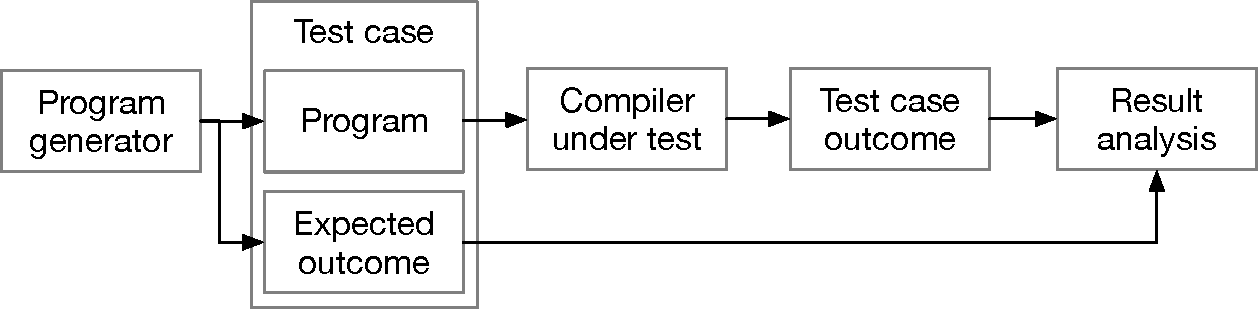
\includegraphics[width=.8\columnwidth]{img/oracle-generator}%
    \label{fig:test-case-generators-oracle}%
  }%
  \\*
  \subfloat[][Differential test case generation and evaluation]{%
    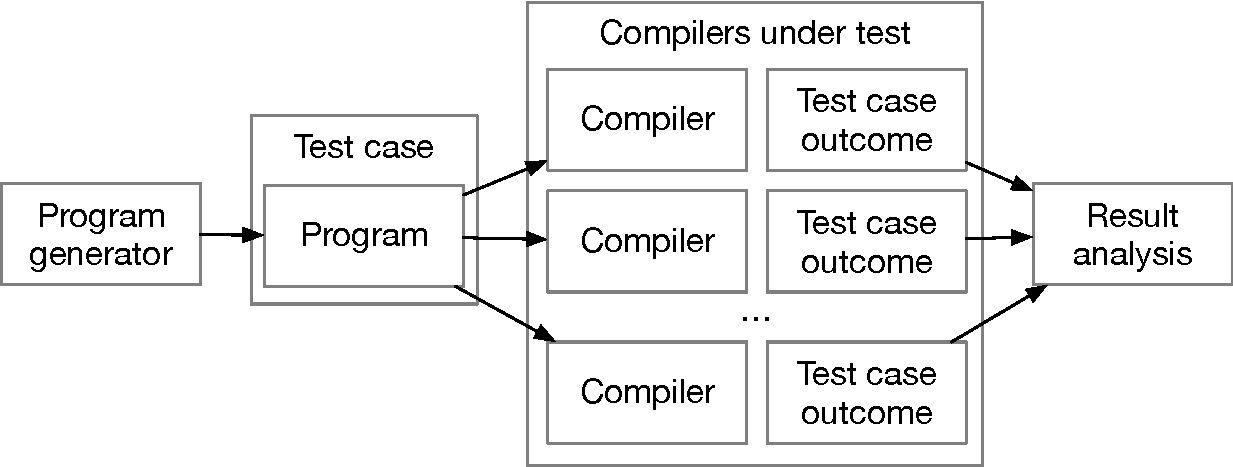
\includegraphics[width=.8\columnwidth]{img/difftest-generator}%
    \label{fig:test-case-generators-difftest}%
  }%
  \caption[Generating and evaluating compiler test cases]{%
    Two approaches to addressing the \emph{compiler validation} problem through test case generation. In~\protect\subref{fig:test-case-generators-oracle}, a test case is composed of a program and a summary of its expected behaviour. In~\protect\subref{fig:test-case-generators-difftest}, only a program is required, and the expected outcome is determined by majority voting on the observed outcomes across multiple compilers.%
  }%
  \label{fig:test-case-generators}
\end{figure}

Differential testing, illustrated in Figure~\ref{fig:test-case-generators-difftest}, accelerates testing by enabling many compilers to be tested at once. In differential testing, a single program is fed through multiple compilers to produce corresponding executables. Each of these executables are run and their outputs recorded. Since the executables were compiled from the same input program, if any of the outputs differ, a bug in one of the compilers has been exposed. The advantage of differential testing over prior approaches is that it does not require a gold standard for the expected behaviour of a conformant compiler. As such, any well-formed program may be used as a test. Even malformed inputs may be used to identify anomalies in the error handling logic of compilers. While lacking a gold standard for behaviour makes differential testing theoretically insufficient to prove that a compiler with a minority output is at fault, in practice the likelihood of the majority consensus being incorrect is extremely unlikely, and no work in the literature has reported such issues.

Differential testing has been applied across different compilers~\cite{Chen2016b,Lidbury2015a} and using the same compiler with different configurations~\cite{Kyle2015b,Paka2011} (and combinations of the two). \citeauthor{Chen2014a}~\cite{Chen2014a} empirically contrasts the two approaches, along with a comparison to Equivalence Module Inputs testing (described in the following subsection).

% McKeeman, W. M. (1998). Differential Testing for Software. DTJ, 10(1).
In the foundational work on differential testing for compilers, \citeauthor{McKeeman1998}~\cite{McKeeman1998} presents generators capable of enumerating programs of a range of qualities, from random ASCII sequences to C model conforming programs. Subsequent works have presented increasingly complex generators which improve in some metric of interest, generally expressiveness or probability of correctness.

% Yang, X., Chen, Y., Eide, E., & Regehr, J. (2011). Finding and Understanding Bugs in C Compilers. In PLDI. https://doi.org/10.1145/2345156.1993532
CSmith~\cite{Yang2011} is a widely known and effective generator which enumerates programs by pairing infrequently combined language features. In doing so, it produces correct programs with clearly defined behaviour but extremely unlikely functionality, increasing the chances of triggering a bug. Achieving this required extensive engineering work, most of it not portable across languages, and ignoring some language features.
% Lidbury, C., Lascu, A., Chong, N., & Donaldson, A. (2015). Many-Core Compiler Fuzzing. In PLDI.
\citeauthor{Lidbury2015a}~\cite{Lidbury2015a} extend CSmith to the OpenCL programming language, a superficially simple task, yet this required 9 man-months of development and 8000 lines of code.
% Nagai, E., Hashimoto, A., & Ishiura, N. (2013). Scaling up Size and Number of Expressions in Random Testing of Arithmetic Optimization of C Compilers. In SASIMI.
Subsequent generators influenced by CSmith focus on compiler features and bug types beyond the scope of CSmith, such as Orange3~\cite{Nagai2013} which targets arithmetic bugs.

% Bastani, O., Sharma, R., Aiken, A., & Liang, P. (2017). Synthesizing Program Input Grammars. In PLDI. https://doi.org/10.1145/3062341.3062349
Similarly to program generation for test compilers, prior work has focused on input generation for testing programs~\cite{Godefroid2005,Claessen2014,Duregard2012,Fetscher2015a,Runciman2008}. Glade~\cite{Bastani2017} derives a context-free grammar for structured program inputs from a corpus of examples. The derived grammar is enumerated to produce new inputs, though no distribution is learned over the grammar; enumeration is uniformly random.

% \diff{Functional programming languages often minimise the use of mutable state and side effects, making them particularly amenable to random testing. \emph{Quickcheck}~\cite{Claessen2000} leverages user-provided code properties to enumerate random test inputs.}

Programs generated by grammar-based approaches are often unlike real handwritten code, and are typically large. As such, once a bug has been identified, test case reduction~\cite{Regehr2012a} is required to minimise the size of the program and isolate the code of interest. Automated test case reduction does not scale to the rate at which effective compiler fuzzers produce programs of interest, often taking minutes or hours for each test case~\cite{Pflanzer2016}.

Entirely machine learning-based approaches to program generation have recently been proposed. They are reviewed in Section~\ref{subsec:related-work-neural-program-generation}.


\subsubsection{Program Mutation and Feedback-directed Compiler Testing}

An alternate method for generating programs to use as compiler test cases is to mutate a seed input.
% Le, V., Afshari, M., & Su, Z. (2014). Compiler Validation via Equivalence Modulo Inputs. In PLDI. https://doi.org/10.1145/2594291.2594334
Equivalence Modulo Inputs (EMI) testing, introduced by~\citeauthor{Le2013a}~\cite{Le2013a}, starts with an existing program and inserts or deletes statements that will not be executed so that the functionality of the code is unchanged. If the functionality of the compiled code is affected, it is due to a bug in the compiler. In the original work~\cite{Le2013a}, code from dead regions is randomly deleted.
% V. Le, C. Sun, and Z. Su, “Finding Deep Compiler Bugs via Guided Stochastic Program Mutation,” in OOPSLA, 2015.
\emph{Athena}~\cite{Le2015} guides the approach using a Markov Chain Monte Carlo method, and supports dead code insertion as well as removal.
% V. Le, C. Sun, and Z. Su, “Randomized Stress-testing of Link-Time Optimizers,” in ISSTA, 2015.
\emph{Proteus}~\cite{Le2015b} applies the EMI technique to test link-time optimisers.
% C. Sun, V. Le, and Z. Su, “Finding Compiler Bugs via Live Code Mutation,” in OOPSLA, 2016.
\emph{Hermes}~\cite{Sun2016a} extends EMI to permit the mutation of \emph{live code} regions, not just dead code. This greatly increases the expressiveness of the generated programs.

\emph{LangFuzz}~\cite{Holler2012} also uses program mutation but does this by inserting code segments which have previously exposed bugs. This increases the chances of discovering vulnerabilities in scripting language engines.
% Peng, H., Shoshitaishvili, Y., & Payer, M. (2018). T-Fuzz: Fuzzing by Program Transformation. In SP.
Starting with a coverage-guided set of inputs, \emph{T-Fuzz}~\cite{Peng2018} uses dynamic tracing to detect input checks in programs and selectively removes them to expose defects.
% Zhang, Q., Sun, C., & Su, Z. (2017). Skeletal Program Enumeration for Rigorous Compiler Testing. In PLDI.
\emph{Skeletal program enumeration}~\cite{Zhang2017a} again works by transforming existing code. It identifies algorithmic patterns in short pieces of code and enumerates all the possible permutations of variable usage.
% Mathis, B., Kampmann, A., Gopinath, R., Höschele, M., Mera, M., & Zeller, A. (2019). Parser-Directed Fuzzing. In PLDI.
\emph{pFuzzer}~\cite{Mathis2019} targets input parsers, using dynamic tainting to produce a set of legal inputs that cover all conditions during parsing.
% Chen, Y., Su, T., Sun, C., Su, Z., & Zhao, J. (2016). Coverage-Directed Differential Testing of JVM Implementations. In PLDI.
Coverage-directed mutation techniques have been used for differential testing the Java Virtual Machine~\cite{Chen2016b}.

Machine learning has been used to guide test case mutation.
% Cheng, L., Zhang, Y., Zhang, Y., Wu, C., Li, Z., Fu, Y., & Li, H. (2019). Optimizing seed inputs in fuzzing with machine learning. ArXiv:1902.02538.
\citeauthor{Cheng2019}~\cite{Cheng2019} construct artificial neural networks to discover correlations between PDF test cases and their execution in the target program. The correlations are then leveraged to generate new paths in the target program.
% She, D., Pei, K., Epstein, D., Yang, J., Ray, B., & Jana, S. (2018). NEUZZ: Efficient Fuzzing with Neural Program Learning. ArXiv:1807.05620.
\emph{NEUZZ}~\cite{She2018} learns a differentiable neural approximation of target program logic, then uses Stochastic Gradient Descent to guide program mutation.
% Wang, J., Chen, B., Wei, L., & Liu, Y. (2017). Skyfire: Data-Driven Seed Generation for Fuzzing. In S&P. https://doi.org/10.1109/SP.2017.23
\emph{Skyfire}~\cite{Wang2017c} learns a probabilistic context-sensitive grammar over a corpus of programs to generate input seeds for mutation testing. The generated seeds are shown to improve the code coverage of AFL~\cite{Zalewski} when fuzzing XSLT and XML engines. The seeds are not directly used as test cases.

EMI and feedback-directed approaches rely on having a large number of seed programs to mutate. As such, they may still require an external code generator. Similarly to grammar-based approaches, these methods often tend to favour large test programs.


\subsubsection{Neural Program Generation}
\label{subsec:related-work-neural-program-generation}

Recently, machine learning methods have been proposed for generating test cases. These differ from prior works that use machine learning to \emph{guide} the generation of test cases.
% Jozefowicz, R., Vinyals, O., Schuster, M., Shazeer, N., & Wu, Y. (2016). Exploring the Limits of Language Modeling. arXiv:1602.02410.
Methods have been proposed based on the success of Recurrent Neural Networks (RNNs) at modelling sequential data~\cite{Jozefowicz2016a}. RNNs have been successfully applied to a broad range of generative tasks in other domains, including image captioning~\cite{Vinyals}, colourising black and white photographs~\cite{Zhang2016}, artistic style~\cite{Gatys2015}, and image generation~\cite{Gregor2014}.

% Sutskever, I., Vinyals, O., & Le, Q. V. (2014). Sequence to Sequence Learning with Neural Networks. In NIPS.
The proficiency of RNNs for sequence modelling is well demonstrated~\cite{Sutskever2014}. \citeauthor{Sutskever2014} apply two RNN networks to translate first a sequence into a fixed length vector, then to decode the vector into an output sequence. This architecture achieves state-of-the-art performance in machine translation. The authors find that reversing the order of the input sequences markedly improves translation performance by introducing new short term dependencies between input and output sequences.

% Neelakantan, A., Le, Q. V., & Sutskever, I. (2016). Neural Programmer: Inducing Latent Programs with Gradient Descent. In ICLR.
Although nascent, the use of artificial neural networks to generate programs is evolving rapidly. \emph{Neural Programmer}~\cite{Neelakantan2016} is an early example of program generation through the latent representation of an artificial neural network.

% Godefroid, P., Peleg, H., & Singh, R. (2017). Learn&Fuzz: Machine Learning for Input Fuzzing. In ASE.
%
% % Nasrabadi, M. Z., Parsa, S., & Kalaee, A. (2018). Neural Fuzzing: A Neural Approach to Generate Test Data for File Format Fuzzing. ArXiv:1812.09961.
\emph{Learn\&Fuzz}~\cite{Godefroid2017} and \emph{IUST DeepFuzz}~\cite{Nasrabadi2018} use LSTM networks, trained on a corpus of PDF files, to generate test inputs for PDF renderers. In the case of \emph{Learn\&Fuzz}, they uncover a bug in the Microsoft Edge renderer. Unlike compiler testing, PDF test cases require no inputs and no pre-processing of the training corpus.

\citeauthor{Jitsunari2019}~\cite{Jitsunari2019} incorporate coverage directed feedback during the training of generative models for PDFs. They train a model on an initial corpus, then sample it. They then evaluate the samples using code coverage and select those that provide the best coverage to be used as additional training data to fine-tune the model. Doing so improves the code coverage of the final generative model.

% Liu, X., Li, X., Prajapati, R., & Wu, D. (2019). DeepFuzz: Automatic Generation of Syntax Valid C Programs for Fuzz Testing. In AAAI.
Most similar to the work presented in this thesis is \emph{DeepFuzz}~\cite{Liu2019}, in which an LSTM network is used to generate fragments of C programs that are inserted into GCC unit tests. The mutated unit tests are then used for differential testing. They propose a character-level model with three sampling methodologies: one where a sample is made for every character, one where no sampling is made (so the generated fragment is conditioned solely on the sample prefix), and a hybrid approach in which sampling occurs only on white-space. In their evaluation, they uncover 8 bugs in GCC, and achieve up to an 82.63\% rate of syntactically valid samples. The work presented in this thesis differs in several ways. The key difference is the use of a recurrent neural network to generate only \emph{fragments} of a program, derived from an existing GCC unit test. In contrast, the approach presented in this thesis generates entire programs. Further, it is trained on a wide range of handwritten programs with the intent of emulating \emph{natural} programming styles.

% Kosta, L., Seaman, L., & Xi, H. (2019). Program Synthesis and Vulnerability Injection Using a Grammar VAE. Journal of Software, 14(6).
\citeauthor{Kosta2019}~\cite{Kosta2019} generate C functions to augment the training dataset of machine learning for static analysis, using vulnerability injection to produce positive examples. They generate programs using a Grammar Variational Autoencoder, an artificial neural network architecture which decomposes a program to a sequence of context-free grammar production rules. Unlike the syntactic-level approach presented in this work, this grammar-based approach guarantees the generation of syntactically correct code by masking production rules that would lead to invalid programs. The authors combine this with semantic repair to further reduce the chance of a sample being invalid.

A drawback of Grammar Variational Autoencoder approaches is the explosion in vocabulary size arising from using a context-free grammar to model a programming language. To mitigate this, the authors must limit the expressiveness of the generator by using only a small subset of the programming language's features. \citeauthor{Kosta2019} achieve this by selecting a handful of C functions to derive a grammar from, followed by further manual pruning of the derived grammar based on what the authors felt would be used most often by programmers. It is unclear whether such an approach could be extended to match the expressiveness of the method presented in this work.

Neural program generation has been used for purposes other than program generation, reviewed in Section~\ref{sec:related-work-other}.


\section{Program Optimisation}
\label{sec:related-work-optimisation}

Modern compilers are complex, typically containing dozens or hundreds of independent optimisation passes. Determining which optimisation passes to apply, and in what order, is a challenge that depends on a variety of factors from the properties of the program being compiled to the target hardware. Current state-of-practice is for compilers to use a fixed ordering of optimisations, and for each optimisation to contain heuristics to determine when the optimisation is applied, and with what parameters. Such heuristics require expert design at the expense of great effort and compiler expertise. Still, they rarely are capable of extracting all of the available performance.

% Georgiou, K., Blackmore, C., Xavier-de-Souza, S., & Eder, K. (2018). Less is More: Exploiting the Standard Compiler Optimization Levels for Better Performance and Energy Consumption. In SCOPES.
Extracting the maximum performance of a program is not simply a case of enabling more optimisations, but in identifying which, out of a set of candidate optimisations, will provide the best performance for the current case. A recent study by \citeauthor{Georgiou2018}~\cite{Georgiou2018} illustrates the scale of the challenge. Using two modern releases of the industry-standard LLVM compiler, they obtain an average 3.9\% performance improvement across 71 benchmarks on embedded processors by selectively \emph{disabling} optimisations enabled at the standard \texttt{-O2} optimisation level.

% Ryoo, S., Rodrigues, C. I., Baghsorkhi, S. S., Stone, S. S., Kirk, D. B., & Hwu, W. W. (2008). Optimization principles and application performance evaluation of a multithreaded GPU using CUDA. In PPoPP.
Selecting the right optimisations is critical. In some domains, the margin of performance to be gained is significant. For example, \citeauthor{Ryoo2008a}~\cite{Ryoo2008a} find speedups of up to $432\times$ through the appropriate selection and use of tiling and loop unrolling optimisations on a GPU matrix multiplication implementation.

Given the challenges of heuristic and analytical methods for extracting performance, researchers have turned to empirical methods such as iterative compilation.


\subsection{Iterative Compilation and Auto-tuning}

Iterative compilation is a method of performance tuning in which a program is compiled and profiled using multiple optimisation configurations to find the configuration which provides the best performance. Unlike analytical methods which attempt to predict the parameters that produce good performance, iterative compilation is empirical. A set of candidate configurations are selected, and for each, the program is compiled and profiled. The configuration that minimises the value of a suitable cost function (such as program runtime) is selected. Pioneered by \citeauthor{Bodin1998}~\cite{Bodin1998}, the technique was initially demonstrated to find good configurations in the non-linear three-dimensional optimisation space of a matrix multiplication benchmark. By exhaustively enumerating the optimisation space they were able to find the global minima of the cost function; however, the authors state that in practice this may not be possible. In cases where an exhaustive enumeration of the optimisation space is infeasible, the process may be cast as a search problem.

While conceptually simple, the empirical nature of iterative compilation yields good results. Iterative compilation has since been demonstrated to be a highly effective form of empirical performance tuning for selecting compiler optimisations.
% Chen, Y., Huang, Y., Eeckhout, L., Fursin, G., Peng, L., Temam, O., & Wu, C. (2010). Evaluating Iterative Optimization Across 1000 Data Sets. In PLDI.
In a large scale evaluation across 1000 data sets, \citeauthor{Chen2010}~\cite{Chen2010} found iterative compilation to yield speedups in GCC over the highest optimisation level (\texttt{-O3}) of up $2.23\times$.

The greatest challenge of iterative compilation is the exponential blow-up of optimisation space size with the addition of independent optimisations. The hundreds of discrete optimising transformations found in modern compilers render an exhaustive search of the optimisation space infeasible. This has driven the development of methods for reducing the cost of evaluating configurations. These methods reduce evaluation costs either by pruning the size of the optimisation space and performing a random or exhaustive enumeration or by guiding a directed search to traverse the optimisation space while evaluating fewer points.


\subsubsection{Pruning the Iterative Compilation Search Space}

% Triantafyllis, S., & August, D. I. (2003). Compiler Optimization-Space Exploration. In CGO. IEEE.
\citeauthor{Triantafyllis2003}~\cite{Triantafyllis2003} propose using feedback during the evaluation of configurations to prune the optimisation space. This is combined with a static performance estimator to obviate the need to run each configuration of a program. \citeauthor{Pan2006}~\cite{Pan2006} formalise the iterative compilation problem as: given a set of compiler optimisation options, find the combination that minimises the program execution time efficiently, without a priori knowledge of the optimisations and their interactions. Their technique, \emph{Combined Elimination}, iteratively prunes the search space, reducing the tuning time to 57\% of the closest alternative. Posing the problem as a subset search negates the challenge of optimisation \emph{ordering}, though this challenge has been the focus of other work~\cite{Kulkarni2012,Purini2013}.

% Ryoo, S., Rodrigues, C. I., Stone, S. S., Baghsorkhi, S. S., Ueng, S., Stratton, J. A., & Hwu, W. W. (2008). Program optimization space pruning for a multithreaded GPU. In CGO. IEEE. https://doi.org/10.1145/1356058.1356084
\citeauthor{Ryoo2008}~\cite{Ryoo2008} prune the optimisation space for GPGPU workloads using the common subset of optimal configurations across a set of training examples. This technique reduces the search space by 98\%. The trade-off of this approach is that there is no guarantee that for a new program, the reduced search space will include the optimal configuration.
% Purini, S., & Jain, L. (2013). Finding Good Optimization Sequences Covering Program Space. TACO.
Similarly, \citeauthor{Purini2013}~\cite{Purini2013} identify a set of good optimisation sequences offline that is small enough for each new program to be tried with all sequences in the set. They find that a sequence set size of 10 yields 13\% speedups on PolyBench and MiBench programs. Although this does not reduce the cost of finding the set of good sequences, the process need only be performed once per platform, so the cost may be amortised by reusing the same sequence set.

Frameworks for iterative compilation offer mechanisms to abstract the iterative compilation process from the optimisation space. These lower the cost of adopting iterative compilation techniques by providing reusable logic to search optimisation spaces. Examples include \emph{OpenTuner}~\cite{Ansel2013} which provides domain-agnostic ensemble search techniques and \emph{CLTune}~\cite{Nugteren2015} for iterative compilation in OpenCL.

A complementary approach to search space pruning is knowledge sharing. The idea is that, since most software has many users, share knowledge of the optimisation space between users rather than having each redundantly perform their own exploration of the optimisation space from scratch. Such ``big data'' approaches to auto-tuning have been variously proposed as
% Fursin, G., & Temam, O. (2010). Collective Optimization: A Practical Collaborative Approach. TACO, 7(4).
\emph{Collective Optimization}~\cite{Saclay2010},
% Memon, A. W., & Fursin, G. (2013). Crowdtuning: systematizing auto-tuning using predictive modeling and crowdsourcing. In PARCO.
\emph{Crowdtuning}~\cite{Memon2013},
% Fursin, G., Miceli, R., Lokhmotov, A., Gerndt, M., Baboulin, M., Malony, A. D., ... Del Vento, D. (2014). Collective Mind: Towards practical and collaborative auto-tuning. Scientific Programming, 22(4).
and \emph{Collective Mind}~\cite{Fursin2014}.
\citeauthor{Fursin2014} argue that the challenges facing widespread adoption of iterative compilation techniques are attributable to: a lack of common, diverse benchmarks and data sets; a lack of common experimental methodology; problems with continuously changing hardware and software; and the difficulty to validate techniques due to a lack of sharing in publications. They propose systems for addressing these concerns which provide a modular infrastructure for sharing iterative compilation performance data and related artefacts across the internet~\cite{Fursin2014}.
% Cummins, C., Petoumenos, P., Steuwer, M., & Leather, H. (2016). Towards Collaborative Performance Tuning of Algorithmic Skeletons. In HLPGPU.
In past work~\cite{Cummins2016}, a domain-specific implementation of knowledge sharing was used to accelerate tuning of stencil codes on GPUs by sharing iterative compilation data between users across the internet.

Other challenges facing iterative compilation are the lack of portability and the inability to respond to change. Any change to the exacting combination of program, input data, and hardware may impact the results of optimisations, invalidating any prior exploration of the optimisation space and requiring a new iterative compilation process to be started from scratch. \emph{Online} techniques attempt to mitigate these issues.


\subsubsection{Online Iterative Compilation}

The expensive optimisation space exploration required by iterative compilation has spurred development of online iterative compilation that interleaves the exploration of the optimisation space with regular program use. This is a challenging task, as a random search of an optimisation space may result in many configurations with performance far from optimal, degrading the quality of service for the user. In a real-world system, evaluating many sub-optimal configurations may cause a significant slowdown of the program. Thus a requirement of dynamic optimisers is that convergence time towards optimal parameters is minimised. Further, \emph{exploration} and \emph{exploitation} must be balanced so as to maintain an acceptable quality of service.

% Tartara, M., & Crespi Reghizzi, S. (2013). Continuous learning of compiler heuristics. TACO, 9(4). https://doi.org/10.1145/2400682.2400705
\citeauthor{Tartara2013}~\cite{Tartara2013} propose a technique for \emph{long-term learning} of compiler heuristics without an initial training phase. They treat the continued optimisation of a program over its lifetime as an evolutionary process with the goal of finding the best set of compiler heuristics for a given binary.

% Ansel, J., & Reilly, U. O. (2012). SiblingRivalry: Online Autotuning Through Local Competitions. In CASES. ACM. https://doi.org/10.1145/2380403.2380425
\citeauthor{Ansel2012}~\cite{Ansel2012} present an adversarial approach to online evolutionary performance tuning. At runtime, the available parallel resources of a device are divided between two partitions. Two configurations of the application are then executed simultaneously, one on each partition. One of the configurations is chosen to be ``safe'', the other, experimental. The configuration which yields the best performance is retained as the ``safe'' choice for future iterations, and the process repeats.

% Mpeis, P., Petoumenos, P., & Leather, H. (2016). Iterative compilation on mobile devices. In ADAPT.
\citeauthor{Mpeis2015}~\cite{Mpeis2015} combine online and offline iterative compilation for mobile devices. They capture slices of user behaviour on a device online during use, which are then replayed offline for iterative compilation. This has the advantage of specialising the performance tuning of software to the behaviour of the individual user.

Related to online iterative compilation is dynamic optimisation. \emph{Dynamo}~\cite{Bala2000} is a dynamic optimiser which performs binary level transformations of programs using information gathered from runtime profiling and tracing. This provides the ability for the program to respond to changes in dynamic features at runtime using low-level binary transformations.


\subsubsection{Algorithmic Choice and Rewriting}

Complementary to iterative compilation is \emph{algorithmic choice}. Like iterative compilation, the goal is to find the configuration of a program that maximises performance. However, whereas iterative compilation indirectly affects the program by selecting compiler optimisations to produce different configurations, algorithmic choice selects between permutations of semantically equivalent algorithms, typically explicitly provided by the user.

\emph{PetaBricks}~\cite{Ansel2009a} is a language and compiler for algorithmic choice. Users provide multiple implementations of algorithms, optimised for different parameters or use cases. This creates a search space of possible execution paths for a given program. This has been combined with auto-tuning techniques for enabling optimised multigrid programs~\cite{Chan2009}, with the wider ambition that these auto-tuning techniques may be applied to all algorithmic choice programs~\cite{Ansel2014}. While this helps produce efficient programs, it places the burden of producing each algorithmic permutation on the developer, requiring them to provide enough contrasting implementations to make a search of the implementation space fruitful.

% Ragan-Kelley, J., Barnes, C., Adams, A., Paris, S., Durand, F., & Amarasinghe, S. (2013). Halide: A Language and Compiler for Optimizing Parallelism, Locality, and Recomputation in Image Processing Pipelines. In PLDI. https://doi.org/10.1016/0024-3205(81)90116-8
\emph{Halide}~\cite{Ragan-Kelley2013} alleviates the burden of algorithmic rewriting by providing a high-level domain-specific language that allows users to express pipelines of stencil computations succinctly.
% Steuwer, M., & Dubach, C. (2017). Lift: A Functional Data-Parallel IR for High-Performance GPU Code Generation. In CGO. IEEE.
The \emph{Lift} framework~\cite{Steuwer2017} uses a set of semantic-preserving rewrite rules to transform high-level Halide-like expressions to candidate low-level implementations, creating a space of possible implementations.


%\subsubsection{Super-optimisation}
%
%An extreme form of iterative compilation is \emph{super-optimisation}. Like with algorithmic choice, the process performs higher-level algorithmic rewrites than compiler transformations. However, the process begins with no description of the algorithm, instead, it typically requires only a handful of input-output examples. Super-optimisation strives to find the \emph{globally} optimal implementation of an algorithm. The term super-optimisation is a reference to the misnaming of compiler \emph{optimisation}, where finding the true optimal is considered an unrealistic goal given the time and resource constraints of a typical compiler.
%
%Pioneered by \citeauthor{Massalin1987}~\cite{Massalin1987}, the smallest possible subroutine which performs a specific function is found through a brute force enumeration of the x86 instruction set. Starting with a program of a single instruction, the super-optimiser tests to see if any possible instruction passes a set of conformity tests. If not, the program length is increased by a single instruction and the process repeats. The optimiser is limited to register-to-register memory transfers, with no support for pointers. This limitation is addressed in \emph{Denali}~\cite{Joshi2002}, a super-optimiser which uses constraint satisfaction and rewrite rules to generate programs which are \emph{provably} optimal, instead of searching for the optimal configuration through empirical testing. Denali first translates a low-level machine code into a guarded multi-assignment form, then uses a matching algorithm to build a graph of all of a set of logical axioms which match parts of the graph before using boolean satisfiability to disprove the conjecture that a program cannot be written in $n$ instructions. If the conjecture cannot be disproved, the size of $n$ is increased and the process repeats.
%% Bunel, R., Desmaison, A., Kumar, M. P., & Torr, P. H. S. (2017). Learning to Superoptimize Programs. In ICLR.
%\citeauthor{Bunel2017a}~\cite{Bunel2017a} formulate code super-optimisation as a stochastic search problem to learn the distribution of different code transformations and expected performance improvement. % As acknowledged by the authors, their approach can be improved by having temporal information of the code structures.
%
%As with iterative compilation, the main problem is in pruning and efficiently navigating the search space. In practice, \citeauthor{Massalin1987}~\cite{Massalin1987} found their system to scale only to subroutines typically fewer than 13 instructions. As such, researchers have turned to machine learning techniques as a means to alleviate the cost of empirical evaluation.


\subsection{Machine Learning for Compiler Optimisations}
\label{subsec:related-work-machine-learning-optimisation}

Machine learning has emerged as a viable means for automatically constructing heuristics for code optimisation. Its great advantage is that it adapts to changes in the software and hardware environments as it has no a priori assumptions about their behaviour.
% Ashouri, A. H., Killian, W., Cavazos, J., Palermo, G., & Silvano, C. (2018). A Survey on Compiler Autotuning using Machine Learning. CSUR, 51(5). https://doi.org/10.1145/3197978
This section provides a brief overview of the field. Comprehensive reviews by \citeauthor{Ashouri2018}~\cite{Ashouri2018} and
% Wang, Z., & O’Boyle, M. (2018). Machine learning in Compiler Optimization. Proceedings of the IEEE, 1(23).
\citeauthor{Zhang2018}~\cite{Zhang2018} provide further detail.

% Agakov, F., Bonilla, E., Cavazos, J., Franke, B., Fursin, G., O’Boyle, M., … Williams, C. K. I. (2006). Using Machine Learning to Focus Iterative Optimization. In CGO. IEEE. https://doi.org/10.1109/CGO.2006.37
Pioneered by \citeauthor{Agakov}~\cite{Agakov}, the application of machine learning to compiler optimisation uses iterative compilation to evaluate a collection of training programs offline and gather features describing the distinguishing properties of the programs. The program features and the optimisation decisions which yield the greatest performance are combined and a model is learned. This model is then used to make predictions on unseen programs by extracting the features describing the program. \citeauthor{Agakov}~\cite{Agakov} use machine learning to guide the iterative compilation search.
% Stephenson, M., Martin, M., & Reilly, U. O. (2003). Meta Optimization: Improving Compiler Heuristics with Machine Learning. In PLDI.
\citeauthor{Stephenson2003}~\cite{Stephenson2003} used ``meta optimisation'' to tune compiler heuristics through an evolutionary algorithm to automate the search of the optimisation space.
% Stephenson, M., Martin, M., & Reilly, U. O. (2003). Meta Optimization: Improving Compiler Heuristics with Machine Learning. In PLDI.
\citeauthor{Kulkarni2012}~\cite{Kulkarni2012} formulate the phase-ordering problem as a Markov process and construct artificial neural networks to predict beneficial optimisation orderings given a characterisation of the state of code being optimised.
% Ashouri, A. H., Bignoli, A., Palermo, G., Silvano, C., Kulkarni, S., & Cavazos, J. (2017). MiCOMP: Mitigating the Compiler Phase-ordering Problem Using Optimization Sub-sequences and Machine Learning. TACO.
\citeauthor{Ashouri2017}~\cite{Ashouri2017} approach the phase-ordering problem by clustering optimisations and using machine learning to predict the speedup of sequences of optimisation clusters.

% Cummins, C., Petoumenos, P., Steuwer, M., & Leather, H. (2015). Autotuning OpenCL Workgroup Size for Stencil Patterns. In ADAPT. Retrieved from http://arxiv.org/abs/1511.02490
%
% Lutz, T., Fensch, C., & Cole, M. (2013). PARTANS: An Autotuning Framework for Stencil Computation on Multi-GPU Systems. TACO, 9(4).
\citeauthor{Lutz2013}~\cite{Lutz2013} and past work~\cite{Cummins2016a} develop domain-specific machine learning systems to optimise stencil computations on GPUs. Restricting the domain of optimisations to a single class of algorithm simplifies the learning task by limiting variance in the range of inputs.
% Ganapathi, A., Datta, K., Fox, A., & Patterson, D. (2009). A Case for Machine Learning to Optimize Multicore Performance. In HotPar.
\citeauthor{Ganapathi2009}~\cite{Ganapathi2009} present an auto-tuner for stencil codes which achieves performance up to 18\% better than that of a human expert. From a space of 10 million configurations, they evaluate the performance of a randomly selected 1500 combinations and use Kernel Canonical Correlation Analysis to build correlations between tunable parameter values and measured performance targets. Performance targets are L1 cache misses, TLB misses, cycles per thread, and power consumption. The use of KCAA restricts the scalability of their system as the complexity of model building grows exponentially with the number of features. In their evaluation, the system requires two hours of compute time to build the KCAA model for only 400 seconds of benchmark data.

% Dastgeer, U., Enmyren, J., & Kessler, C. W. (2011). Auto-tuning SkePU: a Multi-Backend Skeleton Programming Framework for Multi-GPU Systems. In IWMSE. ACM.
A domain-specific machine learning based auto-tuner is presented for the SkePU library in~\cite{Dastgeer2011b}. SkePU is a C++ template library for data-parallel computations on GPUs. The auto-tuner predicts optimal device mapping (i.e.\ CPU, GPU) for a given program by predicting execution time and memory copy overhead based on problem size. Similarly, in this thesis machine learning is used to predict optimal heterogeneous device mapping, though the system is capable of making predictions for arbitrary GPU programs, it is not bound to a single template library.
% Moren, K., & Gohringer, D. (2018). Automatic Mapping for OpenCL-Programs on CPU/GPU Heterogeneous Platforms. In ICCS. https://doi.org/10.1007/978-3-319-93701-4
\citeauthor{Moren2018}~\cite{Moren2018} also tackle the task of mapping arbitrary OpenCL kernels to CPU/GPU using dynamic features extracted from the kernel at runtime.

% TODO:
% \todo[inline]{These three papers:
% % Marco, V. S., Taylor, B., Porter, B., & Wang, Z. (2017). Improving Spark Application Throughput Via Memory Aware Task Co-location: A Mixture of Experts Approach. In Middleware. Retrieved from http://arxiv.org/abs/1710.00610
% \cite{Marco2017}

% % Zhang, P., Fang, J., Tang, T., Yang, C., & Wang, Z. (2018). Auto-Tuning streamed applications on intel xeon phi. IPDPS. https://doi.org/10.1109/IPDPS.2018.00061
% \cite{Zhang2018d}

% % Taylor, B., Marco, V. S., & Wang, Z. (2017). Adaptive Optimization for OpenCL Programs on Embedded Heterogeneous Systems. ACM SIGPLAN Notices, 52(4). https://doi.org/10.1145/3140582.3081040
% \cite{Taylor2017}}

% Fursin, G., Kashnikov, Y., Memon, A. W., Chamski, Z., Temam, O., Namolaru, M., … O’Boyle, M. (2011). Milepost GCC: Machine Learning Enabled Self-tuning Compiler. IJPP, 39(3).
\emph{Milepost GCC}~\cite{Fursin2011} is the first practical attempt to embed machine learning into a production compiler. It adds an interface for extracting program features and controlling optimisation passes, combined with a knowledge sharing system to distribute training data over the internet. The embedded interface exposes candidate features which may be used to apply machine learning to optimisations in GCC.

% Ogilvie, W. F., Petoumenos, P., Wang, Z., & Leather, H. (2017). Minimizing the cost of iterative compilation with active learning. CGO.
\citeauthor{Ogilvie2017}~\cite{Ogilvie2017} use active learning to reduce the cost of iterative compilation by searching for points in the optimisation space which are close to decision boundaries. This reduces the cost of training compared to a random search. The approach complements the techniques presented in this thesis, enabling more efficient use of training data.

Besides compilers, there is a broad range of applications for machine learning in improving software performance.
% Kraska, T., Beutel, A., Chi, E. H., Dean, J., & Polyzotis, N. (2017). The Case for Learned Index Structures. ArXiv:1712.01208.
Surprising applications include the use of machine learning to replace conventional hash functions in key-value stores. \citeauthor{Kraska2017}~\cite{Kraska2017} find that replacing a cache-optimised B-Tree-Index with a deep learning model yields up to 70\% speedups with a $10\times$ reduction in memory on real workloads.
% Krishnan, S., Yang, Z., Goldberg, K., Hellerstein, J. M., & Stoica, I. (2018). Learning to Optimize Join Queries With Deep Reinforcement Learning. ArXiv:1808.03196.
\citeauthor{Krishnan2018}~\cite{Krishnan2018} use deep reinforcement learning to optimise SQL join query implementations. %
When applying machine learning in a new domain, the challenge is often in finding a suitable program representation to use as the features.


\subsubsection{Representing Programs with Features}

The success of machine learning based code optimisation requires having high-quality features that capture the important characteristics of programs. There is an infinite number of potential features, and the suitability of features depends on the application domain and the type of model used. Finding the right set of features to use for a particular case is a non-trivial, time-consuming task.

Various forms of features have been used to summarise programs.
% Dubach, C., Jones, T. M., Bonilla, E. V., Fursin, G., & O’Boyle, M. (2009). Portable Compiler Optimisation Across Embedded Programs and Microarchitectures using Machine Learning. In MICRO. ACM.
\citeauthor{Dubach2009}~\cite{Dubach2009} characterise programs using performance counters.
% Jiang, Y., Zhang, Z. Z., Tian, K., Mao, F., Gethers, M., Shen, X., & Gao, Y. (2010). Exploiting Statistical Correlations for Proactive Prediction of Program Behaviors. CGO. https://doi.org/10.1145/1772954.1772989
\citeauthor{Jiang2010}~\cite{Jiang2010} extract program-level behaviours such as loop trip counts and the size of input files.
% Berral, J. L., Goiri, Í., Nou, R., Julià, F., Guitart, J., Gavaldà, R., & Torres, J. (2010). Towards energy-aware scheduling in data centers using machine learning. In e-Energy. ACM.
\citeauthor{Berral2010a}~\cite{Berral2010a} use additional runtime information such as system load.

In compiler research, the feature sets used for predictive models are often provided without explanation and rarely is the quality of those features evaluated. More commonly, an initially large, high dimensional candidate feature space is pruned through statistical analysis on training programs, or projected into a lower dimensional space.
% Stephenson, M., & Amarasinghe, S. (2005). Predicting Unroll Factors Using Supervised Classification. In CGO. IEEE.
\citeauthor{Stephenson2005}~\cite{Stephenson2005} propose two approaches to select the most useful features from 38 candidates: the first using a Mutual Information Score to rank features, the second using a greedy feature selection.
% Collins, A., Fensch, C., Leather, H., & Cole, M. (2013). MaSiF: Machine Learning Guided Auto-tuning of Parallel Skeletons. In HiPC. IEEE. https://doi.org/10.1109/HiPC.2013.6799098
\citeauthor{Collins2013}~\cite{Collins2013} use Principal Component Analysis (PCA) to reduce a four-dimensional feature space to two dimensions, reducing the size of the space to 0.05\%.
% Dubach, C., Cavazos, J., Franke, B., Fursin, G., O’Boyle, M., & Temam, O. (2007). Fast Compiler Optimisation Evaluation Using Code-Feature Based Performance Prediction. In CF. ACM.
\citeauthor{Dubach2007}~\cite{Dubach2007} also use PCA to reduce the dimensionality of their feature space, but determine the number of components to use such that the selected components account for some fraction of the total variance. In their case, 5 components account for 95\% of the total variance.
% Ting, P., Tu, C., Chen, P., Lo, Y., & Cheng, S. (2016). FEAST: An Automated Feature Selection Framework for Compilation Tasks. ArXiv:1610.09543.
\emph{FEAST}~\cite{Ting2016} combines a range of existing feature selection methods to select useful candidate features.

Prior works have sought to reduce the cost of feature design.
% Park, E., Cavazos, J., & Alvarez, M. A. (2012). Using Graph-Based Program Characterization for Predictive Modeling. In CGO. IEEE.
\citeauthor{Park2012}~\cite{Park2012} present a unique graph-based approach for feature representations. They use a Support Vector Machine (SVM) where the kernel is based on a graph similarity metric. Their technique still requires hand-coded features at the basic block level, but thereafter, graph similarity against each of the training programs takes the place of global features. Being a kernel method, it requires that training data graphs be shipped with the compiler, which may not scale as the size of the training data grows with the number of instances, and some training programs may be large. Additionally, their graph matching metric is expensive, requiring $O(n^3)$ to compare against each training example. This thesis presents techniques to construct machine learning compiler heuristics without the need for program features. These techniques do not need any hand-built static code features, and the deployment memory footprint is constant and prediction time is linear in the length of the program, regardless of the size of the training set.

\newpage
A few methods have been proposed to automatically generate features from the compiler's intermediate representation (IR). These approaches closely tie the implementation of the predictive model to the compiler IR, which means changes to the IR will require modifications to the model.
% Leather, H., Bonilla, E., & O’Boyle, M. (2014). Automatic Feature Generation for Machine Learning Based Optimizing Compilation. TACO, 11(1).
\citeauthor{Leather2014}~\cite{Leather2014} use genetic programming to search for features, requiring a huge grammar to be written, some 160kB in length. Although much of this might be created from templates, selecting the right range of capabilities and search space bias is non-trivial and up to the expert.
% Namolaru, M., Cohen, A., Fursin, G., Zaks, A., & Freund, A. (2010). Practical Aggregation of Semantical Program Properties for Machine Learning Based Optimization. In CASES.
\citeauthor{Namolaru2010a}~\cite{Namolaru2010a} express the space of features via logic programming over relations that represent information from the IRs. They greedily search for expressions that represent good features. However, this approach relies on expert selected relations, combinators and constraints to work. For both approaches, the search time may be significant.

% Cavazos, J., Dubach, C., Agakov, F., Bonilla, E., O’Boyle, M., Fursin, G., & Temam, O. (2006). Automatic Performance Model Construction for the Fast Software Exploration of New Hardware Designs. In CASES.
\citeauthor{Cavazos2006}~\cite{Cavazos2006} present a reaction-based predictive model for software-hardware co-design. Their approach profiles the target program using several carefully selected compiler options to see how a program runtime changes under these options for a given micro-architecture setting. They then use the program ``reactions'' to predict the best available application speedup. While their approach does not use static code features, developers must carefully select a few settings from a large number of candidate options for profiling, because poorly chosen options significantly affect the quality of the model. Moreover, the program must be run several times before optimisation, while the techniques presented in this thesis do not require the program to be profiled.

Compared to these approaches, the techniques presented in this thesis are entirely automatic and require no expert involvement. In the field of compiler optimisations, no work so far has developed deep learning methodologies for program feature generation and selection. This work is the first to do so.


\subsubsection{Distributed Representations for Programs}

This thesis presents deep learning methodologies for learning over programs, inspired by techniques developed in natural language processing. With these techniques, a program source code is tokenised into a sequence of vocabulary words, and each word in the vocabulary is mapped to a real-valued \emph{embedding} space.
There are many choices in how to construct vocabularies and embeddings. \citeauthor{Chen2019}~\cite{Chen2019} review some of the proposed techniques.
% Babii, H., Janes, A., & Robbes, R. (2019). Modeling Vocabulary for Big Code Machine Learning. ArXiv:1904.01873.
\citeauthor{Babii}~\cite{Babii} explore the impact that different permutations of vocabulary make on the convergence time of language models for program code.

% Cvitkovic, M., Singh, B., & Anandkumar, A. (2018). Deep Learning On Code with an Unbounded Vocabulary. Machine Learning, 4.
The techniques in this thesis use a hybrid character/token-level vocabulary to tokenise source code. This is to prevent the blow-up in vocabulary size that occurs from using a purely token-based vocabulary. \citeauthor{Cvitkovic2018a}~\cite{Cvitkovic2018a} propose modelling vocabulary elements as nodes in a graph and then processing the graph using Graph Neural Networks; this enables learning over an unbounded vocabulary.

% Mou, L., Li, G., Zhang, L., Wang, T., & Jin, Z. (2016). Convolutional Neural Networks over Tree Structures for Programming Language Processing. In AAAI.
\citeauthor{Mou2016}~\cite{Mou2016} derive an embedding space from the tokens in the source code of a program.
% Wang, K., Singh, R., & Su, Z. (2017). Dynamic Neural Program Embeddings for Program Repair. ArXiv:1711.07163.
\citeauthor{Wang2017d}~\cite{Wang2017d} propose an embedding space extracted from program traces, rather than the syntactic structure of the program.
% Henkel, J., Lahiri, S. K., Liblit, B., & Reps, T. (2018). Code Vectors: Understanding Programs Through Embedded Abstracted Symbolic Traces. In FSE.
\citeauthor{Henkel2018a}~\cite{Henkel2018a} use symbolic execution to abstract the program traces. Embeddings are then learned from these abstracted symbolic traces.
% Yin, P., Neubig, G., Allamanis, M., Brockschmidt, M., & Gaunt, A. L. (2018). Learning to Represent Edits. ArXiv:1810.13337.
%
% Tufano, M., Pantiuchina, J., Watson, C., Bavota, G., & Poshyvanyk, D. (2019). On Learning Meaningful Code Changes via Neural Machine Translation. ArXiv:1901.09102.
\citeauthor{Yin2018}~\cite{Yin2018} and \citeauthor{Tufano2019}~\cite{Tufano2019} explore techniques for learning embedding representations of code edits.

% Ben-nun, T., Jakobovits, A. S., & Hoefler, T. (2018). Neural Code Comprehension: A Learnable Representation of Code Semantics. In NeurIPS.
\emph{Neural Code Comprehension}~\cite{Ben-nun2018} builds on techniques proposed in Chapter~\ref{chap:deeptune} of this thesis to develop embeddings derived from a novel \emph{Contextual Flow Graph} representation which contains the union of both data and control flow graphs. The embeddings are trained using a skip-gram model~\cite{Mikolov2013a}, using a vocabulary derived from LLVM bitcode. By deriving a vocabulary from a compiler intermediate representation, this enables the same embeddings to be used for any programming language for which there exists a front-end to LLVM.

% TODO: \todo[inline]{There are plenty of other \_2vec papers to touch on}


\section{Deep Learning over Programs}
\label{sec:related-work-other}

% Wang, H., Raj, B., & Xing, E. P. (2017). On the Origin of Deep Learning, 1–81. Retrieved from http://arxiv.org/abs/1702.07800
Deep learning is a nascent branch of machine learning in which deep or multi-level systems of processing layers are used to detect patterns in natural data~\cite{LeCun2015,Wang2017}. Deep learning techniques for program generation and optimisation were reviewed in Section~\ref{subsec:related-work-neural-program-generation} and Section~\ref{subsec:related-work-machine-learning-optimisation} respectively, but there are other applications of deep learning over programs related to this work.

The great advantage of deep learning over prior machine learning techniques is its ability to process natural data in its raw form. This overcomes the traditionally laborious and time-consuming practice of engineering feature extractors to process raw data into an internal representation or feature vector. Deep learning has successfully discovered structures in high-dimensional data and is responsible for many breakthrough achievements in machine learning such as achieving human parity in conversational speech recognition~\cite{Xiong2016}; super-human level performance in video games~\cite{Mnih2015}; and autonomous vehicle control~\cite{Lozano-Perez2012}. The use of deep learning techniques for software engineering has long been a goal of research~\cite{White2015a}.

% Allamanis, M., Barr, E. T., Devanbu, P., & Sutton, C. (2017). A Survey of Machine Learning for Big Code and Naturalness. ArXiv:1709.06182.
A \citeyear{Allamanis2017a} survey by \citeauthor{Allamanis2017a} describes the fast-moving field of deep learning techniques for programming languages~\cite{Allamanis2017a}.
% Wong, E., Yang, J., & Tan, L. (2013). AutoComment: Mining Question and Answer Sites for Automatic Comment Generation. In ASE. IEEE.
\emph{AutoComment}~\cite{Wong2013} mines the popular Q\&A site StackOverflow to automatically generate code comments.
% Allamanis, M., Barr, E. T., Bird, C., & Sutton, C. (2014). Learning Natural Coding Conventions. In FSE. ACM.
\emph{Naturalize}~\cite{Allamanis2014a} employs techniques developed in the natural language processing domain to model coding conventions.
% Raychev, V., Vechev, M., & Krause, A. (2015). Predicting Program Properties from “Big Code.” In POPL. https://doi.org/10.1145/2676726.2677009
\emph{JSNice}~\cite{Raychev2015} leverages probabilistic graphical models to predict program properties such as identifier names for JavaScript.
% Allamanis, M., Peng, H., & Sutton, C. (2016). A Convolutional Attention Network for Extreme Summarization of Source Code. In ICML.
\citeauthor{Allamanis2016}~\cite{Allamanis2016} use attentional neural networks to generate summaries of source code.
% David, Y., Alon, U., & Yahav, E. (2019). Neural Reverse Engineering of Stripped Binaries. ArXiv:1902.09122. Retrieved from https://arxiv.org/pdf/1902.09122.pdf
\emph{Nero}~\cite{David2019} uses an encoder-decoder architecture to predict method names in stripped binaries. The system takes as input a sequence of call sites from the execution of a binary and produces as output a predicted method name.

There is an increasing interest in mining source code repositories at a large scale~\cite{Allamanis2013a,White2015a,Bird2009}. Previous uses outside the field of machine learning have involved data mining of GitHub to analyse software engineering practices~\cite{Wu2014,Guzman2014,Baishakhi2014a,Vasilescu2015}.
% Allamanis, M. (2018). The Adverse Effects of Code Duplication in Machine Learning Models of Code. ArXiv:1812.06469. Retrieved from https://github.com/Microsoft/dpu-utils.
\citeauthor{Allamanis2018}~\cite{Allamanis2018} raises concerns about code duplicates in corpora of open-source programs used for machine learning. They find that corpora often contain a high percentage of duplicate or near-duplicate code. This impacts cases where the corpus is divided into training and test sets. Duplicate code appearing both in the training and test sets leads to artificially high accuracies of models on the test set. The work in this thesis does not use open source corpora as test sets.

Machine learning has also been applied to other areas such as bug detection and static analysis.
% Heo, K., Oh, H., & Yi, K. (2017). Machine-Learning-Guided Selectively Unsound Static Analysis. In ICSE.
\citeauthor{Heo2017}~\cite{Heo2017} present a machine-learning technique to tune static analysis to be selectively unsound, based on anomaly detection techniques.
% Koc, U., Saadatpanah, P., Foster, J. S., & Porter, A. A. (2017). Learning a Classifier for False Positive Error Reports Emitted by Static Code Analysis Tools. In MAPL.
\citeauthor{Koc2017}~\cite{Koc2017} develop a classifier to predict whether the error report produced by a static analysis is a false positive based on the program structures of previous reports that produced false error reports.
% Lam, A. N., Nguyen, A. T., Nguyen, H. A., & Nguyen, T. N. (2015). Combining Deep Learning with Information Retrieval to Localize Buggy Files for Bug Reports. In ASE.
\citeauthor{Lam2016}~\cite{Lam2016} employ artificial neural networks to relate keywords in bug reports to code tokens and terms in source files and documentation to accelerate bug localisation.
% Wang, S., Liu, T., & Tan, L. (2016). Automatically Learning Semantic Features for Defect Prediction. In ICSE. ACM.
\citeauthor{Wang2016c}~\cite{Wang2016c} employ a deep belief network~\cite{Hinton2006a} to automatically learn semantic features from token vectors extracted from the abstract syntax trees of programs. The features are then used for automatic defect detection.
% Chen, J., Bai, Y., Hao, D., Xiong, Y., Zhang, H., & Xie, B. (2017). Learning to Prioritize Test Programs for Compiler Testing. In ICSE.
\citeauthor{Chen2017}~\cite{Chen2017} train two models on compiler test cases, one to predict whether a test case will trigger a compiler bug, the other to predict the execution of the test program. The outputs of these two models are used to schedule test cases so as to maximise the potential for exposing bugs in the shortest amount of time.
% Pradel, M., & Sen, K. (2018). DeepBugs: A Learning Approach to Name-based Bug Detection. In OOPSLA.
\emph{DeepBugs}~\cite{Pradel2018} combines a binary classification of correct and incorrect code with semantic processing to name bugs.
% Si, X., Dai, H., Raghothaman, M., Naik, M., & Song, L. (2018). Learning Loop Invariants for Program Verification. In NeurIPS.
\emph{Code2Inv}~\cite{Si2018} uses reinforcement learning to learn loop invariants for program verification.

% Monperrus, M. (2018). Automatic Software Repair: a Bibliography. CSUR, 51(1).
Machine learning has been applied to the task of automatic software repair. \citeauthor{Monperrus2018} surveys the literature~\cite{Monperrus2018}.
% White, M., Tufano, M., Martínez, M., Monperrus, M., & Poshyvanyk, D. (2019). Sorting and Transforming Program Repair Ingredients via Deep Learning Code Similarities. In SANER.
\emph{DeepRepair}~\cite{White2019} using an encoder-decoder architecture to sort code fragments according to their similarity to suspicious elements.
% Vasic, M., Kanade, A., Maniatis, P., Bieber, D., & Singh, R. (2019). Neural Program Repair by Jointly Learning to Localize and Repair. In ICLR.
\citeauthor{Vasic2019}~\cite{Vasic2019} train a model to jointly localise and repair variable-misuse bugs using multi-headed pointer networks.
% Chen, Z., Kommrusch, S., Tufano, M., Pouchet, L., Poshyvanyk, D., & Monperrus, M. (2018). SequenceR: Sequence-to-Sequence Learning for End-to-End Program Repair. ArXiv:1901.01808. Retrieved from http://arxiv.org/abs/1901.01808
\emph{SequenceR}~\cite{Chen2018} uses sequence-to-sequence learning to generate patches.
% Bader, J., Scott, A., Pradel, M., & Chandra, S. (2019). Getafix: Learning to Fix Bugs Automatically. ArXiv:1902.06111.
\emph{Getafix}~\cite{Bader2019} uses a hierarchical clustering algorithm that summarises fix patterns into a hierarchy ranging from general to specific patterns.
% Brockschmidt, M., Allamanis, M., Gaunt, A. L., & Polozov, O. (2018). Generative Code Modeling with Graphs.
\citeauthor{Brockschmidt2018}~\cite{Brockschmidt2018} present a novel methodology for program generation in which a graph is used as the intermediate representation.

% Terence, P., & Vinju, J. (2016). Towards a Universal Code Formatter through Machine Learning. In SLE.
\emph{CodeBuff}~\cite{Terence2016} uses a hand-designed set of features to learn abstract code formatting rules from a representative corpus of programs.
% Raychev, V., Vechev, M., & Yahav, E. (2014). Code Completion with Statistical Language Models. In PLDI. https://doi.org/10.1145/2594291.2594321
\citeauthor{Raychev2014}~\cite{Raychev2014} use statistical models to provide contextual code completion.
% Gu, X., Zhang, H., Zhang, D., & Kim, S. (2016). Deep API Learning. In FSE. ACM.
\citeauthor{Zhang2015a}~\cite{Zhang2015a} use deep learning to generate example code for APIs as responses to natural language queries.
% Oda, Y., Fudaba, H., Neubig, G., Hata, H., Sakti, S., Toda, T., & Nakamura, S. (2015). Learning to Generate Pseudo-Code from Source Code Using Statistical Machine Translation. In ASE. IEEE.
\citeauthor{Oda2015}~\cite{Oda2015} employ machine translation techniques to generate pseudo-code from source code.


\section{Summary}
\label{sec:related-work-summary}

This chapter has surveyed the relevant literature in the fields of program generation, program optimisation, and the rapidly evolving application of deep learning for programming languages. The next chapter presents a novel technique to improve the performance of machine learning for compiler heuristics by generating executable benchmarks using models trained on corpora of example programs.
